\documentclass[a4paper]{article}
\usepackage{Sweave}
\usepackage{fixltx2e}

\usepackage[margin=1.0in]{geometry}

 \DefineVerbatimEnvironment{Sinput}{Verbatim} { frame = lines, fontshape = sl}
\DefineVerbatimEnvironment{Soutput}{Verbatim}{frame=lines, fontshape = sl}

\title{Prime Without Retrieval: Analysis}
\author{Abhilasha Kumar}

\begin{document}
\Sconcordance{concordance:PrimeWithoutRetrieval_Analysis.tex:PrimeWithoutRetrieval_Analysis.Rnw:%
1 10 1 1 11 10 1 1 2 4 0 1 2 2 1 1 3 2 0 1 3 1 0 1 3 %
1 0 1 4 6 0 1 3 3 1 1 3 1 0 1 1 1 2 4 1 3 0 1 2 2 1 1 %
6 9 0 1 2 2 1 1 14 1 12 2 1 1 19 1 12 1 1 1 6 2 1}

 \maketitle

%\section{Reading File}

\section {Analysing Retrieval States}

First read the file into an object. If you already have the object, then you don't need to worry about this step:

\begin{Schunk}
\begin{Sinput}
> prime_without = read.csv("Compiled_AllSubjects.csv", header = TRUE, sep = ",")
\end{Sinput}
\end{Schunk}

Next, we calculate mean number of states at different levels. Print each object out to see what it contains.  

\begin{Schunk}
\begin{Sinput}
> meanstates = group_by(prime_without, TargetQuestion.RESP.Trial.)%>%
+     summarise(count = n())
> meanstates_persubject = group_by(prime_without, Subject, TargetQuestion.RESP.Trial.)%>%
+     summarise(count = n())
> meanstates_prime =  group_by(prime_without, PrimeCondition, TargetQuestion.RESP.Trial.)%>%
+     summarise(count = n())
> meanstates_persubject_prime =  group_by(prime_without, Subject, PrimeCondition, 
+                                         TargetQuestion.RESP.Trial.)%>%
+     summarise(count = n())
> 
\end{Sinput}
\end{Schunk}

\section {Plotting States per Prime Condition}

First, we make some changes to our variable and condition names so that they are easy to plot:
\begin{Schunk}
\begin{Sinput}
> colnames(meanstates_prime) = c("PrimeCondition", "State", "Count")
> colnames(meanstates_persubject_prime) = c("Subject", "PrimeCondition", "State", "Count")
> meanstates_prime$State = as.factor(meanstates_prime$State)
> meanstates_prime$State = sub("1", "1_Know", meanstates_prime$State)
> meanstates_prime$State = sub("2", "2_DontKnow", meanstates_prime$State)
> meanstates_prime$State = sub("3", "3_Other", meanstates_prime$State)
> meanstates_prime$State = sub("4", "4_TOT", meanstates_prime$State)
\end{Sinput}
\end{Schunk}

Next, we plot the mean number of states per prime condition. We use the group() argument in ggplot to do this:

\begin{Schunk}
\begin{Sinput}
> ggplot(meanstates_prime, aes(x = PrimeCondition, y = Count, fill = State, group = State))+
+  geom_bar(stat = "identity", position = "dodge", width = 0.5)+
+  theme_few()+
+   xlab("Prime Condition") + ylab("Mean Accuracy") + 
+   ggtitle("Number of States by Prime Condition")
\end{Sinput}
\end{Schunk}
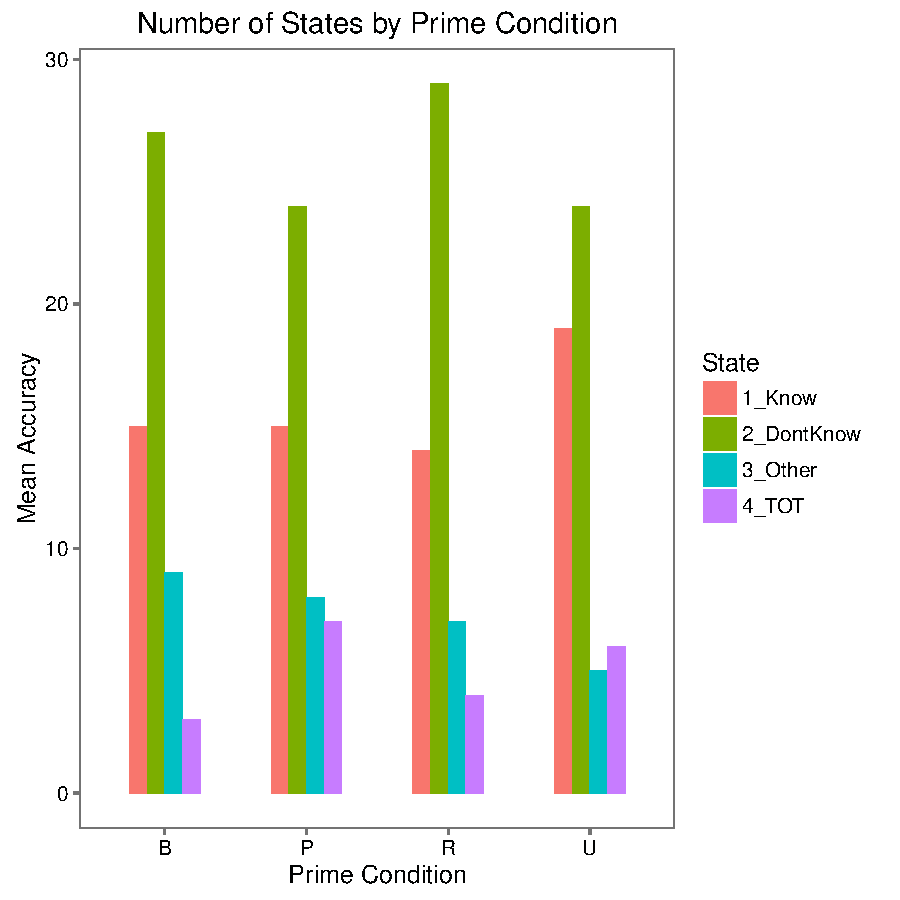
\includegraphics{PrimeWithoutRetrieval_Analysis-005}

%\section {ANOVA on States}



%\section {Actual Plots}



%\section{Linear Model}


\end{document}
